\documentclass[a4paper,12pt,pagesize,headsepline,bibliography=totoc,titlepage]{scrartcl}
\usepackage[utf8]{inputenc}
% \usepackage[T1]{fontenc}
\usepackage{mathptmx}
\usepackage[scaled=.90]{helvet}
\usepackage{courier}
\usepackage{amsmath,amsthm,amsfonts,graphicx,caption}
\usepackage{hyperref}
\usepackage{ae,aecompl}
\usepackage{todonotes}
\usepackage{subcaption}
\usepackage{listings}

\lstset {
	backgroundcolor=\color{white},
	breakatwhitespace=false,
	breaklines=true,
	numbers=left,
	frame=single,
	title=\lstname,
	basicstyle=\footnotesize
}

% \pagestyle{headings}
\headsep4mm % Abstand der Kopfzeile vom Text
% \typearea[current]{current}

\title{
	\includegraphics*[width=0.4\textwidth]{img/hpi_logo.png}\\
	\vspace{24pt}
	Sentence Boundary Detection
}
\subtitle{
	Seminar\\
	Practical Applications of Multimedia Retrieval\\
	Fall Semester 2015/2016
}
\author{
	Tanja Bergmann, Joseph Bethge, Stefan Bunk, Ricarda Schüler\\[12pt]
	Supervisor:\\
    Xiaoyin Che\\
	Dr. Haojin Yang\\
	Prof. Dr. Christoph Meinel
}
\date{\today}

\begin{document}
\maketitle
\tableofcontents
\newpage

\section{Introduction}
\label{sec:introduction}
Automatic Speech Recognition (ASR) has many practical applications nowadays, e.g., in dictation systems for medical documentation and journalism.
Another application comes from the rapidly increasing amount of videos available online on video platforms for entertainment and learning, such as Youtube\footnote{\url{youtube.com}}, Vimeo\footnote{\url{vimeo.com}}, Coursera\footnote{\url{coursera.org}} or OpenHPI\footnote{\url{open.hpi.com}}.
All of these benefit from automatically generated transcripts and subtitles.
But, the result of many ASR systems is an unformatted, long text without punctuation marks, such as periods and commas.
These texts are hard to read, understand, and use without manually inserting the missing punctuation marks.
Therefore, formatting the ASR output and inserting punctuation marks is mandatory for many further use cases.
For example, most machine translation outputs are trained on proper formatted text.
So, having a ASR output without punctuation marks decreases the performance of the machine translating system.
Also other natural language processing task work on sentence units.
Thus, the ASR output needs to be formatted before it can be further processed.

In this paper we want to address this problem by automatically creating punctuated text from unpunctuated text.
We use the concept of deep neural networks to process the unformatted transcript as well as the speech, which results in two individual models: a lexical model and a acoustics model.
We train both models independently and retrieve their separate predictions.
Afterwards the results are combined in a fusion step.
The final output can replace the original output from ASR systems and improve readability and quality of transcripts.
Additionally, the punctuation marks often represent suitable boundaries for subtitles, enhancing their overall quality.

The rest of the paper is structured as follows:
Related work is summarized in Section~\ref{sec:related_work}.
Section~\ref{sec:training_data} describeds the datasets we use for training and evaluation.
The data preprocessing, training, and evaluation of our lexical and our acoustic model can be seen in Section~\ref{sec:lexical_model} and Section~\ref{sec:acoustic_model} respectively.
Details of the fusion step are explained in Section~\ref{sec:fusion}.
We show our demo application in Section~\ref{sec:demo} and conclude our work in Section~\ref{sec:future}.


\section{Related Work}
\label{sec:related_work}

\subsection{Punctuation Prediction}
There are some researcher that focused on pure lexical based punctuation prediction.

Gravano, Jansche und Bacchiani used a simple language model with n-grams to detect punctiations. 
They differed the n-grams between 3 and 6 and evaluated the size of the trainings set. 
They mainly used news articles as data. They found out that about 5-grams and the most data they could get, performed best.
The result is a precision value for comma of 0.55 and for period of 0.65. 
The recall value is 0.68 (comma) and 0.62 (period) \cite{gravano09}. 


Another more advanced method is dynamic conditional random fields. 
Lu and Tou Ng used adoption of this method to predict punctuations in transcripts of dialogs in Chinese and English, which means many short sentences and more than usual questions. 
They were able to outperform hidden event language model \cite{Lu_betterpunctuation}.

\cite{DBLP:conf/interspeech/UeffingBV13} also used dynamic conditional fields. They evaluated this method with different features like language model scores, parse trees, dynamic sentence length and token n-grams. 
They discovered that the usefullness of the features differs to the used texts. If the text is more structured then the parse tree features are useful, for TED-Talks for example they did not help much.


Ein Abschnitt für lexical, eines für acoustic.
Welche Features?
Welchen Grundalgorithmus? (SVM, Decision Tree?)
Deren Ergebnisse.



\subsection{Distributed Representations}
word2vec
\subsection{Caffe}


\section{Training Data}
\label{sec:training_data}
% how did we prepare our data

Our data set, which is used to predict punctuations, can be separated into to parts:
The first part is based on TED talks\footnote{\url{ted.com}}, the second part is a subset from Wikipedia\footnote{\url{en.wikipedia.org}}.

\paragraph{TED talks} Our TED talk data set consists of TODO talks. For each talk we have the following data files:
\begin{itemize}
	\item \texttt{.xml} file: This file contains a manually created script of the talk.
	The text is formatted and serves as training data for the lexical model.
	\item \texttt{.ctm} file: This is a time-marked speech input.
	It contains one word per line with the second the word was said in the talk and its duration.
	Additionally, each sentence is labeled in the file, so that the data can be used for training of the acoustic model.
	\item \texttt{.sph} file: This file contains pulse code modulation (PCM) data.
	This data can be converted into .wav files.
\end{itemize}

\paragraph{Wikipedia} We used a small subset of the English Wikipedia to obtain more training data.
We selected only those articles with more than 10,000 characters.
Besides, we extracted the plain text of the articles, discarding lists, headlines, tables, etc.
In total we received around 3.5 million new training instances from the Wikipedia articles.


\section{Lexical Model}
\label{sec:lexical_model}
In this chapter we describe how we predict the position of periods, commas and question marks in unpunctuated text using lexical features.
The used data is described in Section \ref{sec:training_data}.

% TODO: use
%\begin{figure}[ht]
%    \centering
%    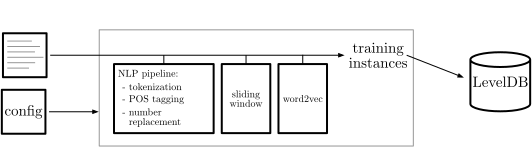
\includegraphics[width=\textwidth]{img/overview_lexical.pdf}
%    \caption{}
%    \label{fig:overview_lexical}
%\end{figure}

The system is based on the deep learning framework \emph{caffe}.
Therefore the processing pipeline is the following:

\begin{itemize}
\item preprocess the data, so that it can be used as input for caffe
\item train the network with the preprocessed data
\item retrieve predictions for new data
\item transform the output into a valuable result
\end{itemize}

\subsection{Data Preprocessing}

For processing the data, we need to extract features which caffe can handle.
Since you can not use a whole text as input, we decided to use a sliding window to generate training and testing instances.
A sliding window is in our case, that we split a sentence like \emph{The sun is shining and we go outside} into the following pieces (assuming a window size of 5):
\begin{itemize}
\item the sun is shining and
\item sun is shining and we
\item is shining and we go
\item shining and we go outside
\end{itemize}

% TODO: use
%\begin{figure}[ht]
%    \centering
%    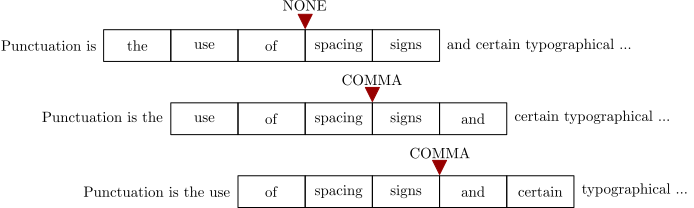
\includegraphics[width=\textwidth]{img/sliding_window.pdf}
%    \caption{}
%    \label{fig:sliding_window}
%\end{figure}

We call these pieces instances and the window size directly defines how many words are in each instance.
The label of each instance is then whether there is a punctuation (and which one) at a defined position.
We call this position punctuation position.
In the above example every instance would have a label of \emph{None} with a punctuation position of 2, since there is no punctuation.

After we split up the sentences into instances we convert each word into a distributed word representation.
We use the distributed word representation described earlier: \emph{word2vec}. \todo{Insert word2vec link. Describe Word2Vec in related work?}
The final model we used for our distributed word representation was trained on google news entries \todo{Link and/or paper}.
Since not every word exists in the trained model, we use the word vector representing \emph{this} for unknown words.
We think that most of the unknown words are proper names, which can easily be replaced with \emph{this} without changing the meaning and structure of the whole sentence.

We also figured out that the trained model only contains the number \emph{1} and a few more of the most common numbers instead of all numbers. \todo{Check whether only 1 is in the word vector or whether numbers like 12 and 5 are also contained}
That is why we replace any number with \emph{1}.

The representation for each word in an instance is inserted into one row of the feature matrix, e.g. for a sliding window size of 5 you get the matrix of 5x300 for each instance.

Besides the distributed word representation we also examined Part of Speech (POS) tags as features.
We used the nltk POS tagger to identify the POS tags with the whole text as input.
The tagger distinguishes between 35 different POS tags.
These are too specific for our purpose, so we reduced them into 14 different categories.
For example we combined CD and LS to a more generic category \emph{numeral}.
The nltk tagger predicts more than one tag per word, so one word can have multiple tags (even after reducing the tag categories).
To allow the existence of multiple tags in our feature matrix, we used the following representation:
We create one flag per POS category which has the value 1 if the word belongs to this category and 0 otherwise.

There are two possibilities to include them.
On the one hand it is possible to append all flags at the end to word vector representations.
On the other hand an extra channel with the flags can be used.

For all further testing, wherever we used the POS-features, we decided to append the flags to the vector representation of the words.
Therefore the resulting feature matrix for a sliding window size of 5 with POS tags is 5x314.

% Data preparation
% Windowing
% Config.ini File

% Google Vector

\subsection{Neural Network Layout}

We use a neural network layout with three main \texttt{innerproduct} layers with sizes 2048, 4096, and 2048.
After each of these layers we added a \texttt{ReLU} and a \texttt{dropout} layer on top of each \texttt{innerproduct} layer.
The ratio for all \texttt{dropout} layers is $0.5$.
Accuracy and loss of the network are computed after the final predictions of our fourth \texttt{innerproduct} layer wih size 3 or 4 depending on the number of punctuation symbols.

\begin{figure}[ht]
    \centering
    
\includegraphics[width=0.6\textwidth]{img/net_lexical.pdf}
    \caption{Network architecture consisting of four fully connected layers.}
    \label{fig:net_lexical}
\end{figure}

\subsection{Results and Evaluation}

We used the measure of precision \emph{P} and recall \emph{R} as well as the F-Measure. We calculated the F measure per class as shown in Equation \ref{equ:f1n}.
We also calculated the harmonic mean \emph{F} for all classes (None, Comma, Period) (see Equation \ref{equ:f1}). This means the higher that value is the better is it. This score is used in the following diagrams.

\begin{equation}
\label{equ:f1n}
F1_{N} = 2 * \frac{P_{N}* R_{N}}{P_{N}+R_{N}}
\end{equation}

\begin{equation}
\label{equ:f1}
F = \frac{3}{\frac{1}{F1_{None}} + \frac{1}{F1_{Comma}} + \frac{1}{F1_{Period}}}
\end{equation}

All experiments are executed with the previous described data preprocessing and network layout.
As training data we used TED talks, which are not included in the training stets.

\begin{figure}[ht]
    \centering
    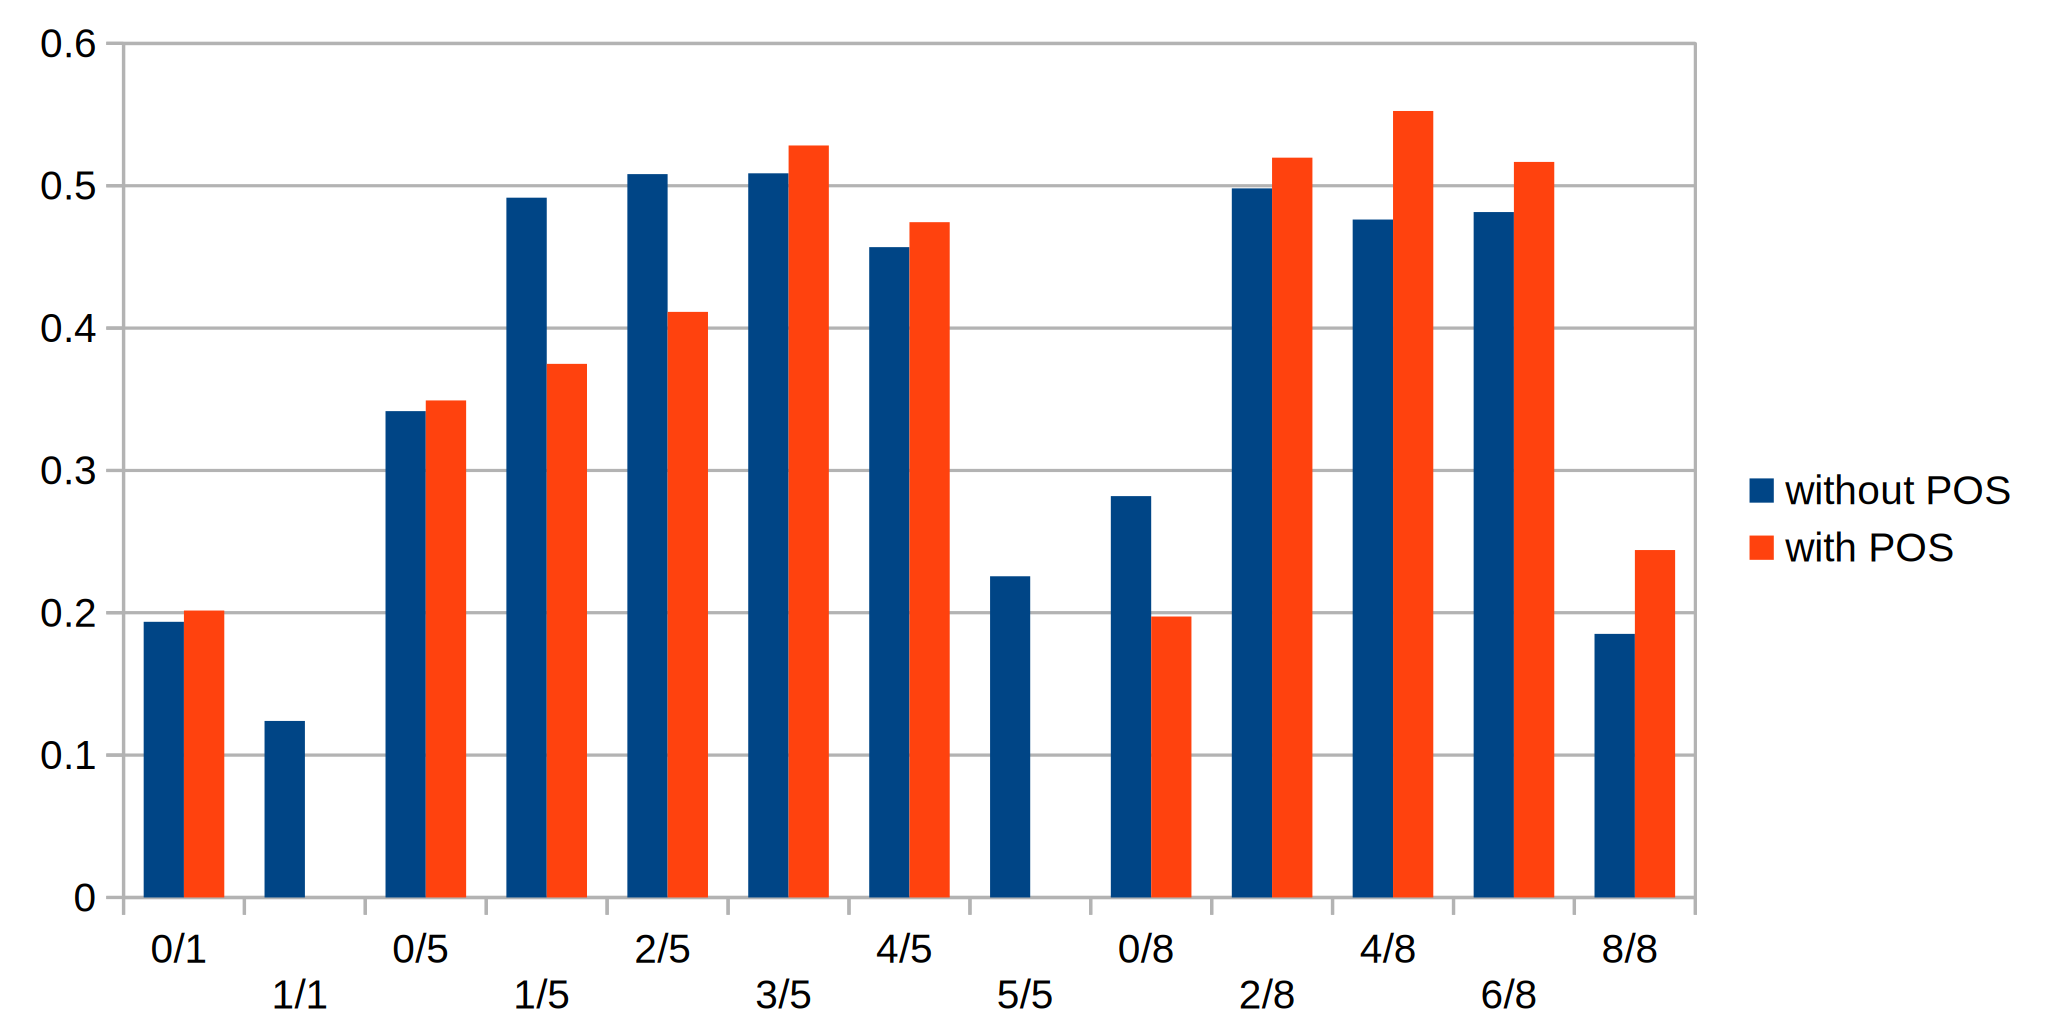
\includegraphics[width=0.9\textwidth]{img/window_eval.png}
    \caption{Harmonic mean between all F1 scores for all classes. \emph{2/5} means window size of five and punctuation position two. If \emph{wi} is in the label, it uses wikipedia training data.}
    \label{fig:window_eval}
\end{figure}

We did experiments do get relations between several parameters.
On the one hand we varied the window size and punctuation position.
In Figure \ref{fig:window_eval} you can see the results.
We found out that the best position for the punctuation is in the middle of the window.
We get the best results for a window size of 8.
This means that more context the better the results, until a certain point.

\begin{figure}[ht]
    \centering
    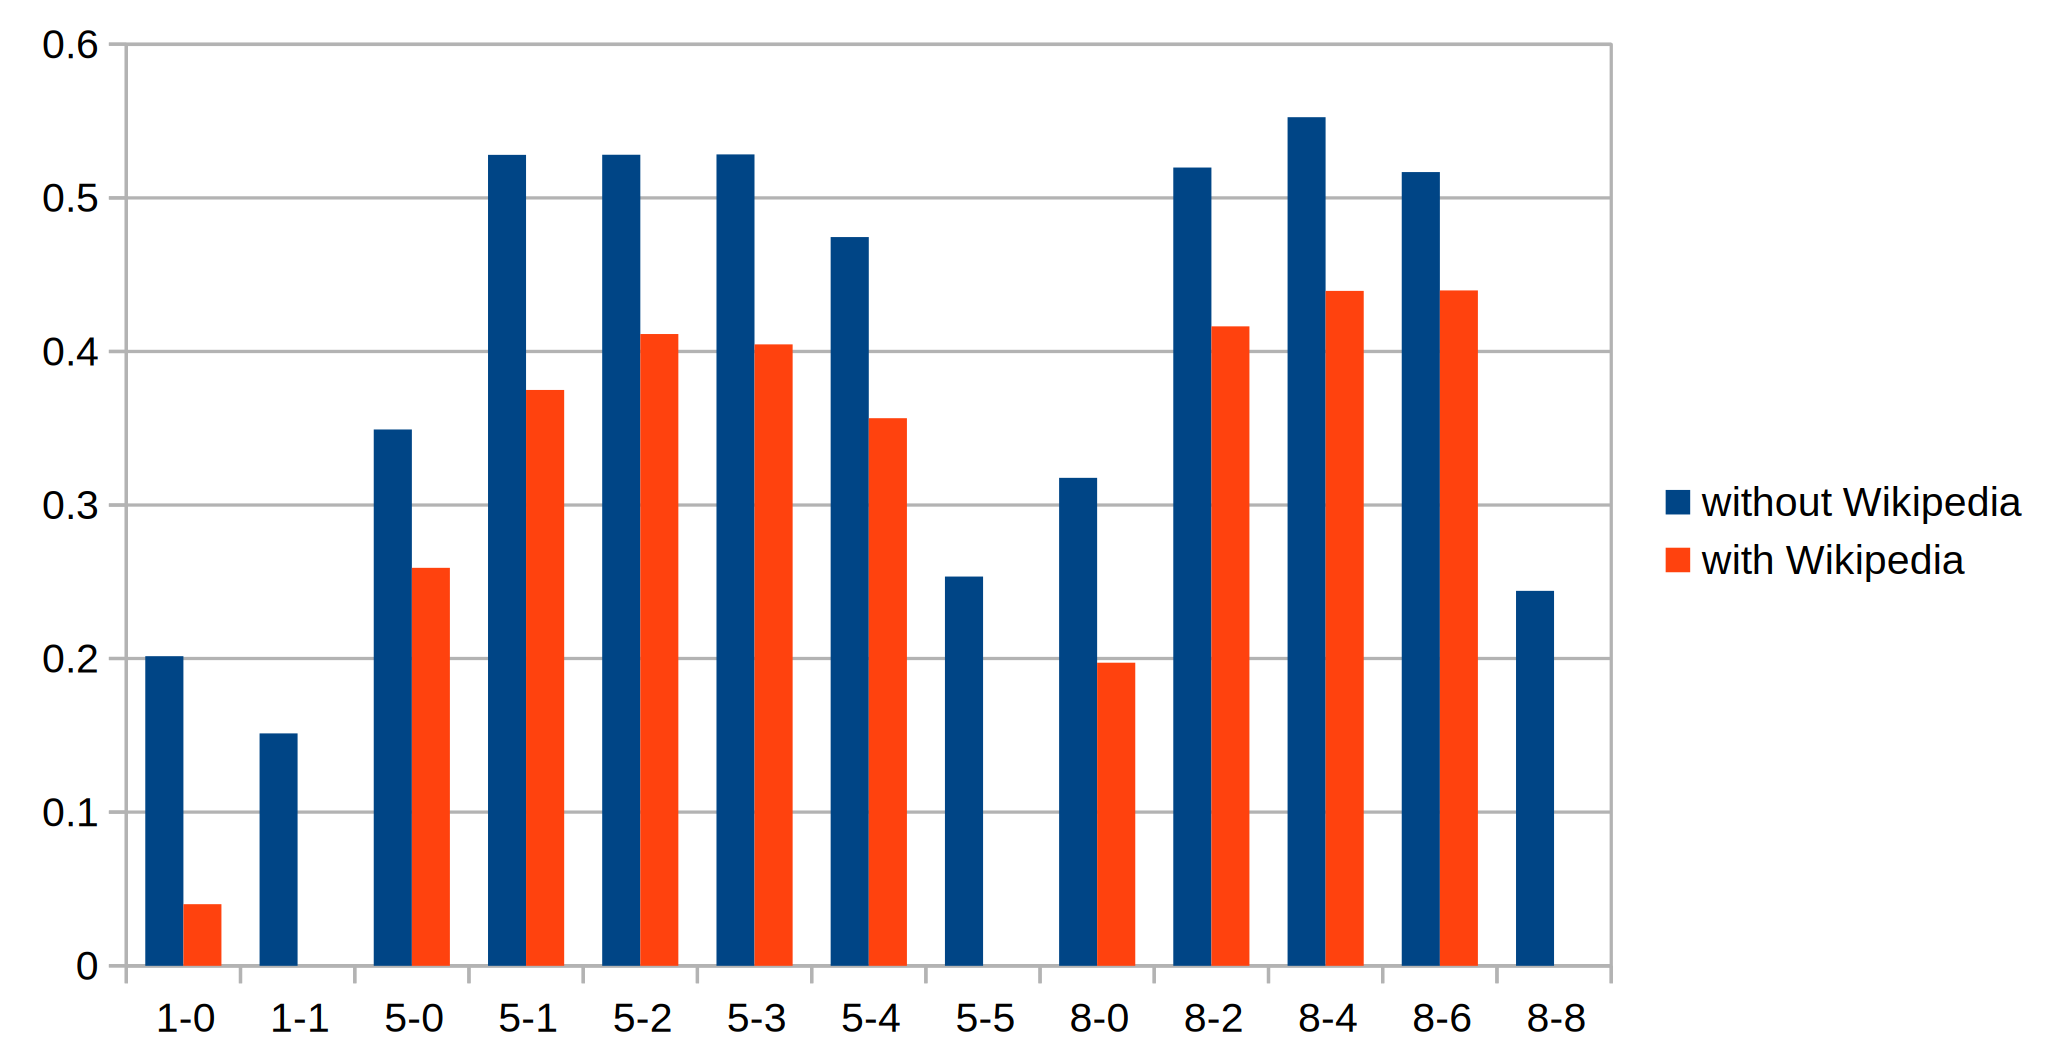
\includegraphics[width=0.75\textwidth]{img/window_wiki_eval.png}
    \caption{F score with different window and punctuation positions. Compares only TED talks and TED talks with additional wikipedia data as training data.}
    \label{fig:window_wiki_eval}
\end{figure}

As described in Section \ref{sec:training_data}, we wanted to use more data for lexical prediction.
In Figure \ref{fig:window_wiki_eval} a comparison between using only TED talks and using additionally wikipedia data as training data is shown.
The described F-score is used, as well as different window sizes and punctuation positions.
The result for varying the window size is the same as described in the experiments above.
You can see that using wikipedia data as additional training data always performs worse.
An experiment without wikipedia data has a F-score of 0.385, whereas the same experiment with wikipedia has only a F-score of 0.252.
This shows that more data does not help in general, although we think that the more data the network learned from the better the results should be.
This result can be explained with the used testing data.
The trained network is evaluated with TED talks.
This is spoken language and wikipedia articles are written language by its nature.
We evaluated the network also with wikipedia data (different from trainings data), which yields to a F-score of 0.60.
This shows that written and spoken language is different, so that predicting punctuations for other language structures does not work that good as for data with the same structure.

\begin{figure}[ht]
    \centering
    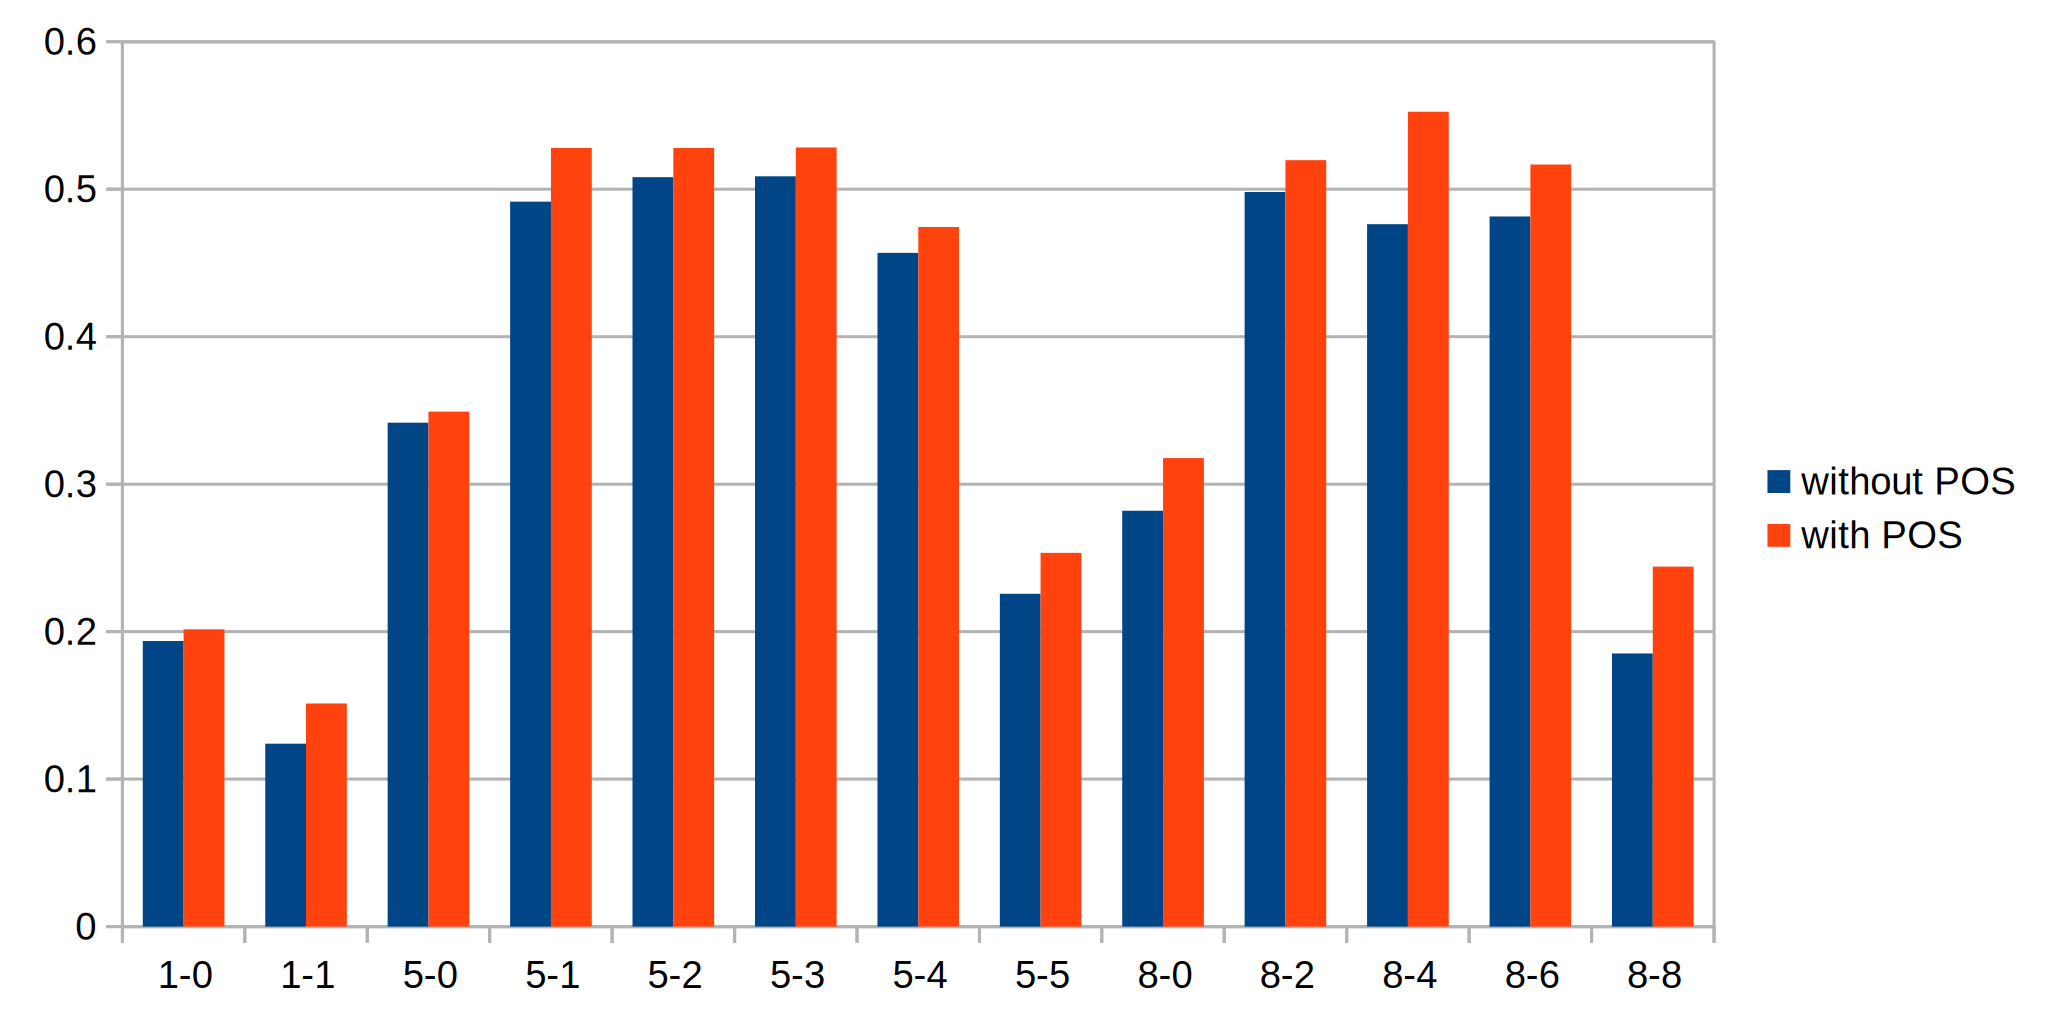
\includegraphics[width=0.75\textwidth]{img/window_pos_eval.png}
    \caption{}
    \label{fig:window_pos_eval}
\end{figure}

We also evaluated if using POS-Tags improves the results. Figure \ref{fig:window_pos_eval} shows the F-score depending on the different window sizes and punctuation positions. The red bars are the results with using the POS-Feature and the blue bars are the result without (the normals one, shown in the other graphs too).
You can see that using the additional POS Feature performs always better.
Compare to experiments with and without POS tagging (other than that, they have the same configurations) with POS tagging has a F-score of 0.305 whereas without POS tagging has only a F-score of 0.275.

Since the punctuation types in the data sets are not equally distributed, we thought about reducing the dataset to a set were the types are balanced. Therefore we created training sets, were nearly equally distributed punctuations types are included. Experiments show that this performs worse as the normal sets. This is likely since the data set is much smaller.


\section{Acoustic Model}
\label{sec:acoustic_model}
\begin{figure}[ht]
    \centering
    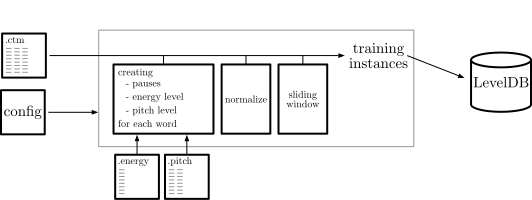
\includegraphics[width=\textwidth]{img/overview_accoustic.pdf}
    \caption{}
    \label{fig:overview_accoustic}
\end{figure}

\begin{figure}[ht]
    \centering
    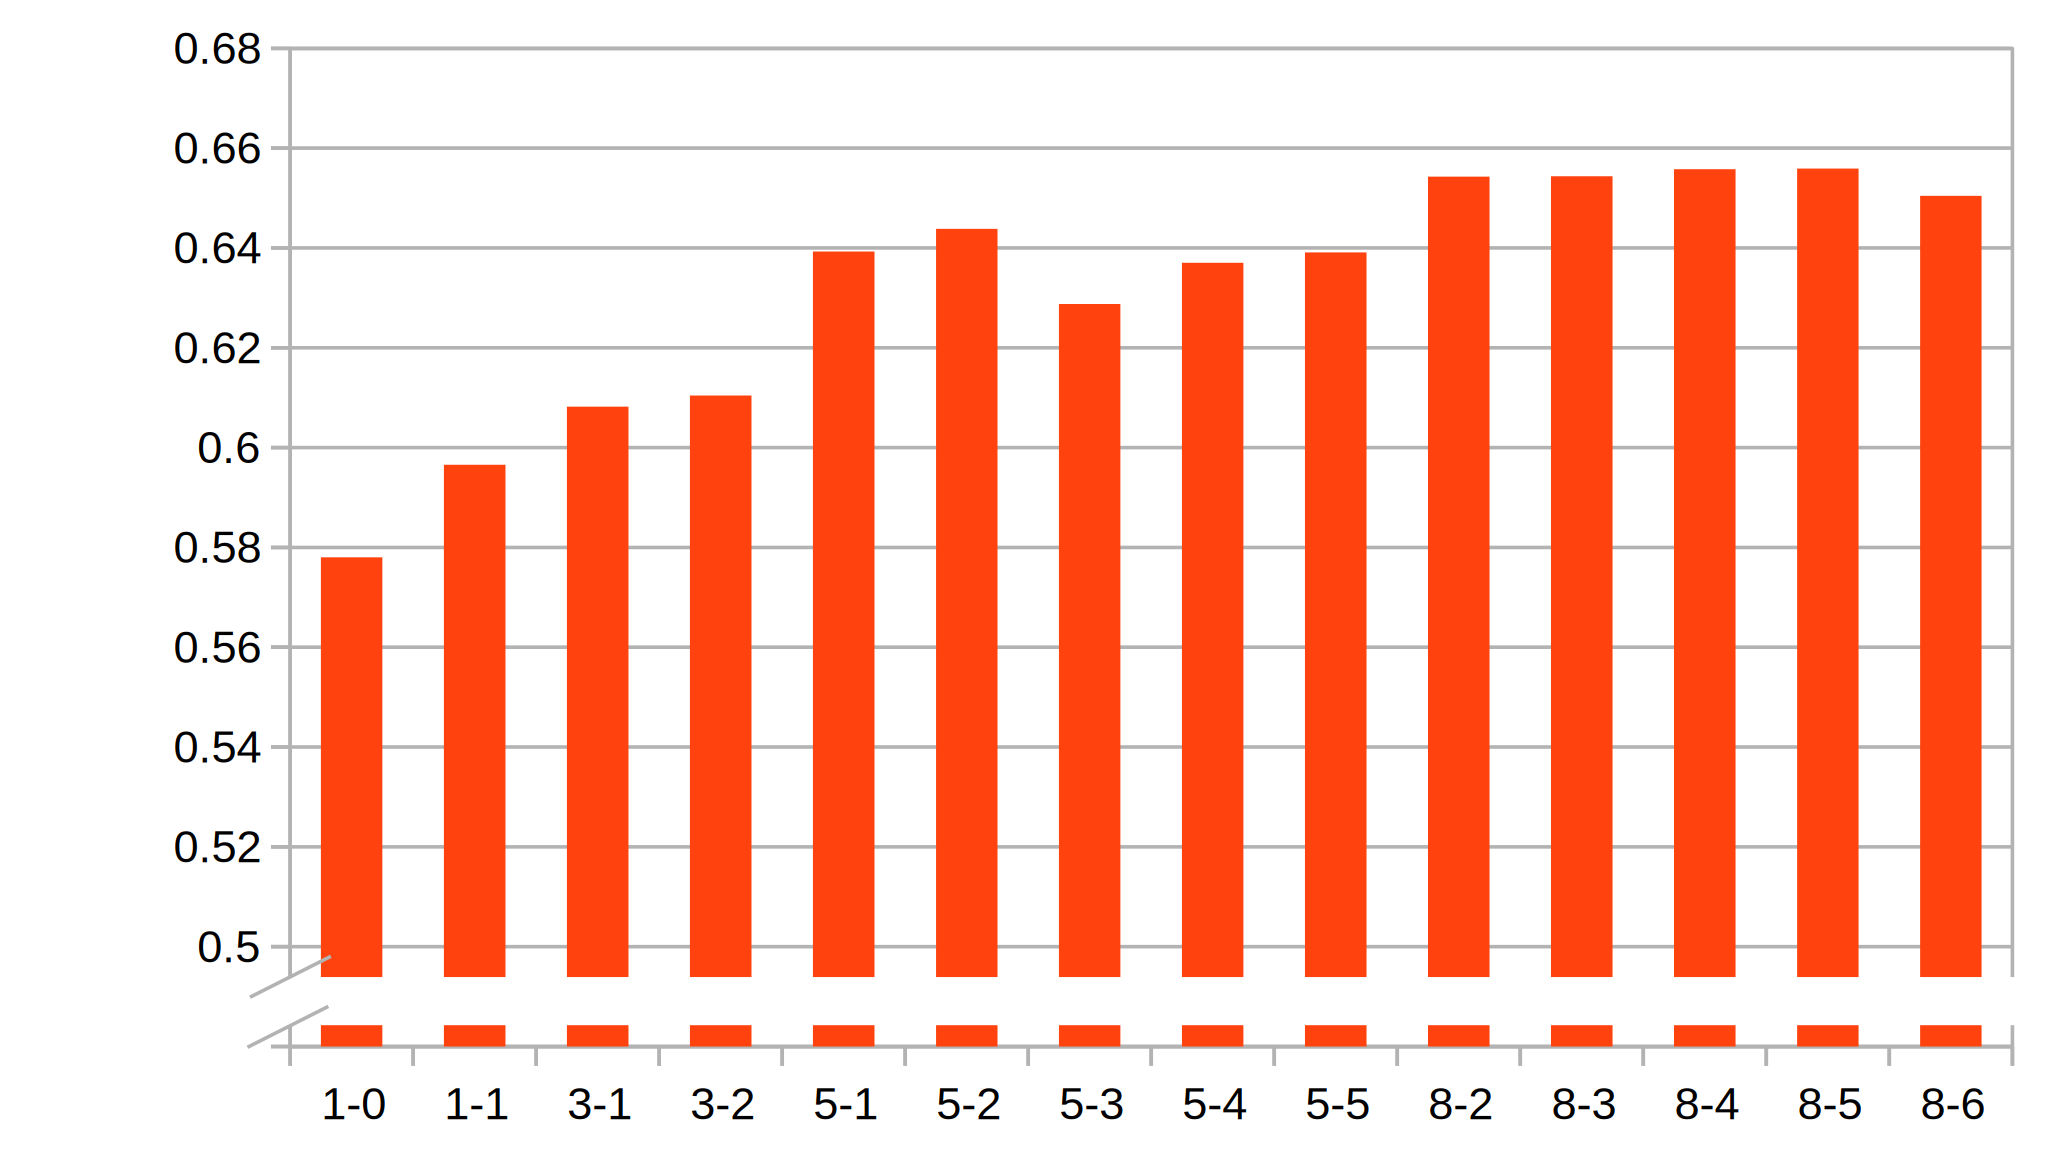
\includegraphics[width=\textwidth]{img/audio_parameter_eval.png}
    \caption{}
    \label{audio_eval}
\end{figure}

\section{Fusion}
\label{sec:fusion}
\begin{figure}[ht]
    \centering
    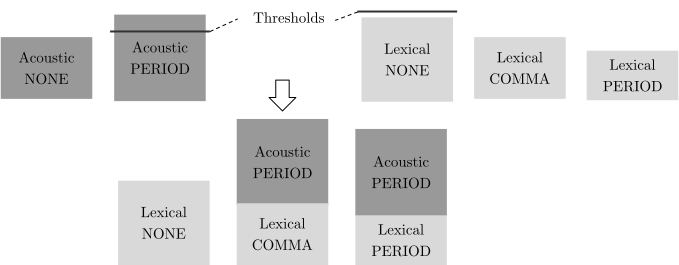
\includegraphics[width=0.7\textwidth]{img/fusion_1.pdf}
    \caption{Network architecture consisting of four fully connected layers of the acoustic model.}
    \label{fig:fusion_1}
\end{figure}

\begin{figure}[ht]
    \centering
    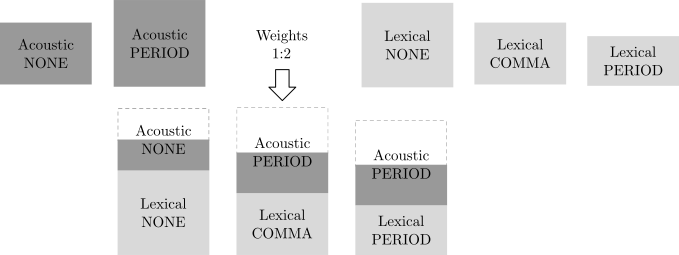
\includegraphics[width=0.7\textwidth]{img/fusion_2.pdf}
    \caption{Network architecture consisting of four fully connected layers of the acoustic model.}
    \label{fig:fusion_1}
\end{figure}

\section{Demo Tool}
\label{sec:demo}
We use a demo application, accessible with a web browser, to present the working prototype.
It can be used to find sentence boundaries in unpunctuated text.
The general web page shows two main tabs, one labeled \emph{Lexical} and one \emph{Lexical + Audio}.
A user can click these, to switch between using only the lexical model or the fusion of both the lexical and the acoustic model.

There are two ways to feed input to our model for the \emph{Lexical} SBD (see Figure~\ref{fig:demo_l}).
\begin{figure}[ht]
    \centering
    \includegraphics[width=0.5\textwidth]{img/demo_l.png}
    \caption{The demo application for lexical model. The results are presented below the options for input and model selection.}
    \label{fig:demo_l}
\end{figure}
The user can enter a text input field to manually enter or paste any text they wish.
Another possibility is to choose from a set of existing text files.
A dropdown selection allows the user to choose the pretrained models, if multiple models are available in the system.
If the model is changed, it is automatically loaded in the background.
Once the user clicks the \emph{Punctuate!} button, the text, which was entered, or selected as a file, is passed to our lexical model.
While the server processes the request, a small loading icon is shown inside the button.
After the predictions are returned from the server, the result is shown beneath.
The input text and positions where no punctuation was predicted are shown as tokens with a light grey background.
Any commas or periods inserted, are shown in distinct colors.
If a model, which uses POS tags, is selected a user can hover their mouse over a token to see its POS category.
For further use the entire result is selectable and can be copied.

For the \emph{Lexical + Audio} SBD the possibilities for entering input are more limited (see Figure~\ref{fig:demo_la}).
\begin{figure}[ht]
    \centering
    \includegraphics[width=0.5\textwidth]{img/demo_l_a.png}
    \caption{The demo application for fusion of both models. The results of the individual models and the fusion are presented below the options for input and model selection. Only one result section is in the screenshot, the other sections are out of the region of the screenshot.}
    \label{fig:demo_la}
\end{figure}
Since we need an audio recording, we offer only examples existing in the system.
At the moment the system contains samples, which were used in the testing phase, but not for training.
The selection of the user is therefore limited by a dropdown menu of all available choices.
However, the choice of both the acoustic and the lexical model is independently available to a user.
These can also be selected in a dropdown menu.
The functionality of the \emph{Punctuate!} button is unchanged.
It triggers the processing and shows a loading indicator until the result returns.
The result area however is changed, and contains three subareas, which each contain a different result.
Two of them contain the raw results of the acoustic model and the lexical model.
The third shows the result after the fusion.
Therefore, it is easy to compare the results of each individual model, and the result after the fusion.

\section{Future Work}
\label{sec:future}
% future work
We showed our approach to automatically detect sentence boundaries, and predict the correct punctuation marks.
Two different models were trained independently, one using lexical input and the other acoustic input.
The results of both models were merged with a late fusion.

There are many possibilties for improvement on the presented approach.
Since we did not explore a large variety of different neural network layouts, further exploration in this area could improve the results.
Especially if combined with more training data a deeper network architecture might improve the quality of the prediction.
Another approach is the usage of Long Short Term Memory (LSTM) in the neural network.

In the fusion step we decided for a late fusion approach, which only combines the predictions.
However another way to explore, is an earlier fusion, where both models and the fusion itself are trained together and the features are fused, instead of the predictions.
As for data preparation, a different representation of features in the lexical model can be examined, such as a second or third data channel or a combination similar to the fusion of the acoustic and lexical model.

The last point for minor improvements could be done with a post processing of the results.
For example, two punctuation symbols with only one or very few words between them is often not correct.


\bibliographystyle{plain}
\bibliography{main.bib}

\newpage
\appendix
\section{Appendix}
We appended the following files for reference:
\begin{itemize}
    \item lexical-solver.prototxt, the configuration of the solver (lexical model)
    \item lexical-net.prototxt, our net configuration (lexical model)
    \item acoustic-solver.prototxt, the configuration of the solver (acoustic model)
    \item acoustic-net.prototxt, our net configuration (acoustic model)
\end{itemize}

\subsection{lexical-solver.prototxt}
\lstinputlisting[caption={lexical-solver.prototxt}, label={lst:lexical-solver.prototxt}]{../net/solver.prototxt}
\newpage

\subsection{lexical-net.prototxt}
\lstinputlisting[caption={lexical-net.prototxt}, label={lst:lexical-net.prototxt}]{../net/net.prototxt}
\newpage

\subsection{acoustic-solver.prototxt}
\lstinputlisting[caption={acoustic-solver.prototxt}, label={lst:acoustic-solver.prototxt}]{../net-audio/solver.prototxt}
\newpage

\subsection{acoustic-net.prototxt}
\lstinputlisting[caption={acoustic-net.prototxt}, label={lst:acoustic-net.prototxt}]{../net-audio/net.prototxt}

%\newpage %for more appended files

\end{document}
